\chapter{过渡元素}
\section{过渡元素概述}\label{sec:Transition_element}
\subsection{过渡元素在元素周期表里的位置和外围电子层排布}
我们从元素周期表上可以看到，表的中部从 \MyRoman{3}B 族 到 \MyRoman{2}B 族 10 个纵行，包括镧系和锕系，共有 68 种元素\footnote{原文是 63 种元素，是按当时已知存在元素为 107 种而计算的。}，这些元素包括了第 \MyRoman{8} 族和全部副族元素，人们习惯上把它们叫做过渡元素。它们分属于第四周期到第七周期，如\cref{fig:1-1} 所示。
\begin{sidewaysfigure}
  \includegraphics{1-1.pdf}
  \caption{过渡元素在元素周期表里的位置}\label{fig:1-1}
\end{sidewaysfigure}

过渡元素原子的电子层排布有共同的特征。
从\cref{fig:1-1} 可以看出,它们的最外电子层都有 \num{1}{2} 个 $s$ 电子（\ce{Pd} 除外），随着原子序数的递增，增加的电子大多填充在次外层的 $d$ 轨道上。
其中镧系和锕系元素的原子，增加的电子主要填充在倒数第三层的 $f$ 的外围电子层排布反映了它不同于主族元素原子的核外电子排布的特征。
例如，钪（\ce{Sc}）的外围电子层排布为 $3d^14s^2$，铀（\ce{U}）的外围电子层排布为 $5f^36d^17s^2$。
过渡元素的许多性质，都跟它们这样的外围电子层排布有关。

\subsection{过渡元素的通性}
\subsubsection{过渡元素都是金属}
过渡元素都是金属，所以人们又把它们叫做过渡金属。
它们原子的最外层电子数不超过 2 个，容易失去，原子间也容易形成金属键，固态时呈金属晶体。
过渡金属的原子跟同周期主族元素的金属原子相比，一般具有较小的原子半径。
过渡金属有较大的密度，较高的熔点和沸点。
例如，铂的密度是 \qty{21.45}{g/cm^3} 约是铝的 8 倍；钨的熔点是 \qty{3410}{\celsius}，是所有金属里最难熔的。

此外，过渡金属还往往具有较高的硬度，较好的延展性和机械加工性能，较好的导电、导热性能和耐腐蚀性能，并且可以组成具有多种特性的合金。
例如金、银等金属有优异的延展性，可以抽成极细的金属丝，轧成极薄的金属箔；银、铜等金属具有良好的导电、导热性能，铂、钛、铬、镍等金属都有良好的耐腐蚀性能，等等。



\subsubsection{过渡元素常有多种可变化合价}
过渡元素在形成化合物时，最外层的 $s$ 电子和次外层的 $d$ 电子等都有可能参加成键。
因此，过渡元素往往有变价。
\cref{tab:1-1} 列出了第四周期过渡元素常见的化合价（下划横线的是比较稳定的价态）。
\begin{table}
  \caption{第四周期过渡元素常见的化合价}\label{tab:1-1}
  \begin{tblr}{colspec={cccX[c]},hline{2}=0.8pt}
    族           & 元素符号 & 外围电子排布 & 化合价 \\
    \MyRoman{3}B & \ce{Sc} & $3d^14s^2$ & $\underline{+3}$ \\
    \MyRoman{4}B & \ce{Ti} & $3d^24s^2$ & $+2\ +3\ \ \underline{+4}$ \\
    \MyRoman{5}B & \ce{V}  & $3d^34s^2$ & $+2\ +3\ +4\ \ \underline{+5}$ \\
    \MyRoman{6}B & \ce{Cr} & $3d^54s^1$ & $+2\ \ \underline{+3}\ \ \underline{+6}$ \\
    \MyRoman{7}B & \ce{Mn} & $3d^54s^2$ & $\underline{+2}\ +3\ \ \underline{+4}\ +6\ \ \underline{+7}$ \\
    \SetCell[r=3]{m,c}\MyRoman{8}  
    &\ce{Fe} & $3d^64s^2$ & $+2\ \ \underline{+3}$\\
    &\ce{Co} & $3d^74s^2$ & $\underline{+2}\ +3$\\
    &\ce{Ni} & $3d^84s^2$ & $\underline{+2}\ +3$\\
    \MyRoman{1}B & \ce{Cu} & $3d^104s^1$ & $+1\ \ \underline{+2}$ \\
    \MyRoman{2}B & \ce{Zn} & $3d^104s^2$ & $\underline{+2}$ \\
  \end{tblr}
\end{table}

从\cref{tab:1-1} 可以看出，从 \MyRoman{3}B 族到 \MyRoman{7}B 族，元素的最高化合价在数值上跟它的族数相等，那是由于这些元素原子的外围电子层的 $s$ 电子和 $d$ 电子数目之和跟族数相等。

\subsubsection{过渡元素的化合物往往带有颜色}

过渡元素的化合物往往带有颜色。
这些颜色跟过渡金属离子的结构有关系，也跟所结合的阴离子的种类、晶体里是否有结晶水等因素有关系。
例如，氟化铜（\ce{CuF2}）是白色的，硫化铜（\ce{CuS}）是黑色的；二氯化钴（\ce{CoCl2}）是蓝色的，六水合二氯化钴（\ce{CoCl2.6H2O}）是粉红色的；无水硫酸铜（\ce{CuSO4}）是白色的，五水合硫酸铜（\ce{CuSO4.5H2O}）是蓝色的。

过渡元素的化合物在水溶液里也往往有颜色，这些颜色是过渡金属水合离子的颜色，水合离子的颜色跟化合物晶体的颜色常常是一致的或者相近的，有时也有所不同。
例如，水合铜离子呈蓝色，跟五水合硫酸铜的颜色一致，但跟无水硫酸铜的颜色就有所不同了。

此外，过渡元素还容易形成络合物。
关于络合物的知识，我们将在\cref{sec:complex}里学习。

\subsection{过渡元素对于国防和国民经济的重要意义}
过渡元素对于国防和国民经济各部门有着极其重要的意义。因为国防和国民经济各部门需要大量的钢铁，同时也需要各种各样的其它过渡金属。例如，电器工业需要大量的铜，电子工业还需要银、金、铂、钯等金属。高速飞机、火箭和舰艇的制造需用钛。铬、锰、镍、锌、钴、钨、钼、钒、铌、钽、镧系元素等，广泛用于生产各种合金或合金钢，而这些合金或合金钢对于制造导弹、坦克、枪炮等武器和各种机器、设备是必不可少的。锕系元素的铀是原子核反应堆的燃料和制造原子弹的材料。多种过渡金属如铂、钯、钒、钛、镍、铁等还是化学工业的重要催化剂。

我国许多过渡元素(例如镧系元素、钨、钼、锰、钒、钛等) 的矿藏十分丰富，这对于我国实现四个现代化是一个有利的条件。

\begin{Practice}[习题]
\begin{question}
  \item 什么叫过渡元素？它们的电子层排布有什么特点？写出铬、锰、钴、镍的电子排布式。
  \item 为什么过渡元素都是金属？它们多数具有哪些共同的物理性质？
  \item 为什么过渡元素常有多种可变化合价？举例说明。
  \item 硅胶（二氧化硅的水合物，又叫硅酸凝胶）是一种干燥剂，里面加有一定量的显色剂 \ce{CoCl2} 以指示吸湿程度。这种干燥剂未吸水时呈蓝色，吸水过多失去干燥能力时呈粉红色。试说明硅胶变色的原因。
  \item 过渡元素对于国防和国民经济具有什么重要意义？
\end{question}
\end{Practice}

\section[络合物]{络合物\texorpdfstring{\protect\footnote{络合物又叫配位化合物。}}{}}\label{sec:complex}
在\cref{sec:Transition_element}里我们已经知道，白色的无水硫酸铜溶于水，它的水溶液呈蓝色，这是铜的水合离子的颜色。
实验测定，铜的水合离子是一种带有 4 个水分子的复杂离子 \ce{[Cu(H2O)4]^2+} 。
下面我们来学习这类复杂离子的知识。

\subsection{络合物的组成}
\subsubsection{络合物的概念}
先做下面的实验。
\begin{Experiment}
在盛有硫酸铜溶液的试管里滴入少量氢氧化钠溶液，生成蓝色的氢氧化铜沉淀；然后滴入适量浓氨水，沉淀消失，得到深蓝色的溶液。再滴入少量氢氧化钠溶液，深蓝色溶液不发生变化，不再生成氢氧化铜沉淀。
\end{Experiment}

现在让我们来分析这个实验所发生的反应。

我们早已知道，硫酸铜跟氢氧化钠起反应能生成氢氧化铜沉淀。
根据物质的溶解性，\ce{Cu(OH)2} 虽然难溶，但终究有一定的溶解度。
因此，\ce{Cu(OH)2} 沉淀跟溶液里微量的 \ce{Cu2+}、\ce{OH-} 之间存在着平衡：
\[ \ce{ Cu(OH)2 <=> Cu^2+ + 2OH- } \]
从分析实验证明，当加入氨水后，\ce{NH3} 分子跟溶液里微量的 \ce{Cu^2+} 结合，在水溶液里生成一种呈深蓝色的复杂离子一 \ce{[Cu(NH3)4]^2+}，它叫四氨合铜（\MyRoman{2}）\footnote{括号内的数字表示化合价}离子或铜氨络离子。这个反应可以用离子方程式表示如下：
\[ \ce{4NH3 + Cu^2+ = [Cu(NH3)4]^2+ }\]
这样就使溶液里存在的 \ce{Cu^2+} 离子浓度降低，从而破坏了 \ce{Cu(OH)2} 跟 \ce{Cu^2+}、\ce{OH-} 之间的平衡，促使 \ce{Cu(OH)2} 沉淀逐渐溶解。
这个反应所生成的 \ce{[Cu(NH3)4]^2+} 在水溶液里较难电离，溶液中存在的 \ce{Cu^2+} 很少。
因此，当再加入少量 \ce{OH-} 时，就不能生成 \ce{Cu(OH)2} 沉淀了。
如果把这种溶液浓缩结晶，我们就可以得到一种深蓝色的晶体—— \ce{[Cu(NH3)4]SO4}，它叫硫酸四氨合铜（\MyRoman{2}）或硫酸铜氨。
硫酸铜氨是一种复杂的化合物，在这种化合物里含有复杂的 \ce{[Cu(NH3)4]^2+}。
这种由一种离子跟一种分子，或由两种不同的离子所形成的一类复杂离子，叫做\Concept{络离子}。
象硫酸铜氨这样含有络离子的化合物，就属于\Concept{络合物}。
上面讲到的 \ce{[Cu(H2O)4]^2+} 也是络离子，含有 \ce{[Cu(H2O)4]^2+} 的胆矾 \ce{CuSO4.5H2O} 是一种络合物。
从前学过的冰晶石 \ce{Na3(AlF6)}（六氟合铝酸钠）也是络合物。

\subsubsection{络合物的组成}
根据研究知道，络合物的结构很复杂，但一般说来，它都有一种成分作为整个络合物的核心，其它成分都围绕这个核心作一定的排列。
例如，在 \ce{[Cu(NH3)4]SO4} 这种络合物里，\ce{Cu^2+} 就是核心，叫做\Concept{中心离子}，4 个 \ce{NH3} 分子均匀地分布在它的周围，叫做络合物的\Concept{配位体}。
中心离子和配位体结合在一起就构成络离子。
\ce{SO4^2-} 距中心离子比较远，跟中心离子的关系不象配位体那么密切。
人们把中心离子和配位体一起构成的络离子叫做络合物的内界（在化学式里常用方括号把它们括起来）；把其它部分如 \ce{SO4^2-} 离子叫做络合物的外界（\cref{fig:1-2}）。

\begin{figure}
  \includegraphics{1-2.pdf}
  \caption{\ce{[Cu(NH3)4]SO4} 的组成示意图}\label{fig:1-2}
\end{figure}

络合物的中心离子，一般都是阳离子。
络合物的配位体可以是分子，也可以是阴离子。
如在 \ce{[Cu(NH3)4]SO4} 里，配位体 \ce{NH3} 是中性分子，在 \ce{Na3[AlF6]}里，配位体 \ce{F-} 是阴离子。
络离子是带电荷的，而络合物呈电中性。
因此，组成络合物的外界离子、中心离子和配位体离子电荷的代数和必定为零。

一个中心离子所能结合的配位体的总数，叫做中心离子的\Concept{配位数}\footnote{严格说来，应是 “一个中心离子（或原子）所能结合的配位体的配位原子（直接同中心离子络合的原子）总数，就是中心离子（或原子）的配位数。”}。在络离子 \ce{[Cu(NH3)4]^2+} 里，\ce{Cu^2+} 的配位数是 4，在 \ce{Na3[AlF6]} 里，\ce{Al^3+} 的配位数是 6。影响中心离子配位数的因素很多，它跟中心离子和配位体的电荷、半径和外围电子层排布等因素都有密切的关系。

\subsubsection{络合物中的化学键}
络合物的各个部分是靠什么键结合起来的呢？根据研究知道，络合物的外界离子跟络离子之间以离子键相结合，中心离子跟配位体之间以配位键相结合。

我们知道，形成配位键必须具有两个前提，一是一方有空轨道，一是另一方能提供孤对电子。
现在来分析 \ce{[Cu(NH3)4]^2+} 里配位键的形成。

\ce{Cu^2+} 的 $3d$ 轨道没有填满，$4s$、$4p$ 轨道的能级跟 $3d$ 轨道相近，它们是空的，所以 \ce{Cu^2+} 有空轨道，而 \ce{NH3} 有一对孤对电子：
\[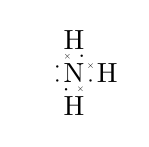
\begin{tikzpicture}[inner sep=1pt]
  \node (c){N};
  \foreach \x in {-1,0,1}
  {
    \node(h\x) at (90*\x:1.2em) {H};
    \draw[draw=none] (c)--(h\x)node[midway,sloped,above,inner sep=1pt]{\scalebox{0.35}{$\times$}}node[midway,sloped,below,inner sep=1pt]{\footnotesize$\cdot$};
  }
  \node(h2) at(180:1.2em){\phantom{H}};
  \draw[draw=none](c)--(h2)node[midway,above,inner sep=0pt]{\footnotesize$\cdot$}node[midway,below,inner sep=1pt]{\footnotesize$\cdot$};
\end{tikzpicture}\]
当 \ce{Cu^2+} 跟 \ce{NH3} 作用时，便以配位键形成了 \ce{[Cu(NH3)4]^2+}：
\[ \left[ 
  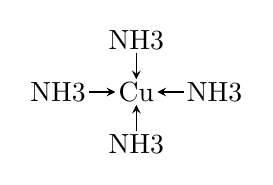
\begin{tikzpicture}[baseline,>=stealth,inner sep=1pt]
    \node (c) {\ce{Cu}};
    \node (u) at (0,0.5) [above]{\ce{NH3}};
    \node (d) at (0,-0.5)[below] {\ce{NH3}};
    \node (l) at (-0.6,0)[left] {\ce{NH3}};
    \node (r) at (0.6,0)[right] {\ce{NH3}};
    \draw[->](u)--(c);
    \draw[->](d)--(c);
    \draw[->](l)--(c);
    \draw[->](r)--(c);
  \end{tikzpicture}
 \right]^{2+}\]

过渡元素离子如 \ce{Fe^3+}、\ce{Fe^2+}、\ce{Cu^2+}、\ce{Ag+}、\ce{Hg^2+} 等都具有空轨道，因此都容易形成络合物，这是过渡元素的特性。
至于 \ce{F-}、\ce{Cl-}、\ce{CN-}、\ce{SCN-} 等阴离子或 \ce{H2O}、\ce{NH3} 等分子都有孤对电子，因而都可以成为配位体。
凡是可作配位体（或含有可作配位体的离子）的物质叫做\Concept{络合剂}。
常用的络合剂有氰化物、氟化物和氨等。

\begin{Reading}{络合物在水溶液里的电离平衡}
络合物的外界跟内界是以离子键结合的，因此，当络合物溶于水时，络合物会发生电离而形成外界和内界两种离子。同时，络离子在水里也会发生一定程度的电离。例如：
\begin{gather*} 
  \schemestart
  \ce{ [Cu(NH3)4]^2+} \arrow(.mid east--.mid west){<=>} \ce{Cu^2+} \+ \ce{4NH3  }
  \schemestop\\ 
  \schemestart
  \chemname{\ce{[Ag(NH3)2]+}}{\footnotesize 二氨合银离子（银氨络离子）}
  \arrow(.mid east--.mid west){<=>} \ce{Ag+} 
  \+ 
  \ce{2NH3}\schemestop\chemnameinit{}\\
  \schemestart
  \chemname{\ce{[Ag(CN)2]-}}{\footnotesize 二氰合银离子（银氰络离子）}
  \arrow(.mid east--.mid west){<=>} \ce{Ag+} 
  \+ 
  \ce{2CN-}\schemestop\chemnameinit{}
\end{gather*}

不同络离子电离程度的大小不同。
一般说来，配位体是 \ce{CN-} 的络离子的电离程度总是很小。
人们利用含氰络离子电离程度很小，即溶液里跟络离子达成平衡的金属离子浓度很小的特点，在电镀工艺中控制金属离子结合电子的速度，从而保证电镀的质量。
所以在电镀工业里配制电镀液时常使用氰化物作络合剂。
但是氰化物有剧毒，因此，现在电镀工业正在研究和使用别的无毒络合剂的无氰电镀工艺。
\end{Reading}


\subsection{络合物的应用}
络合物在自然界广泛存在，跟人类生活的关系很密切。
例如，在人和动物体内起着输送氧气作用的血红素，是 \ce{Fe^2+} 的络合物；在植物生长中起光合作用的叶绿素是含 \ce{Mg^2+} 的络合物。

络合物在工农业生产和科学技术方面的应用也很广泛，例如，在冶金、稀有金属的提取、电镀、照相术等方面都有应用，氰化提金法就是用于稀有金属提取的一个例子。
这个方法的原理是: 用稀的氰化钠溶液处理粉碎了的金矿石，通入空气，使金矿石中的金粒溶解，生成能溶于水的络合物 \ce{Na[Au(CN)2]}：
\[ \ce{4Au + 8NaCN + 2H2O + O2 \xlongequal{\quad} 4Na[Au(CN)2] + 4NaOH} \]
然后再用锌从溶液中把金置换出来：
\[ \ce{ 2Na[Au(CN)2] + Zn \xlongequal{\quad} Na2[Zn(CN)4] + 2Au v} \]

在照相底片和感光纸定影时，需要应用硫代硫酸钠溶液溶解掉未起反应的溴化银，这是一个络合反应，它的化学方程式如下：
\[ \ce{AgBr + 2Na2S2O3 \xlongequal{\quad} Na3[Ag(S2O3)2] + NaBr} \]

在化学实验里，还可以利用形成显色的络离子或络合物来鉴定离子。
例如，利用 \ce{SCN-} 跟 \ce{Fe^3+} 反应生成红色的硫氰合铁（\MyRoman{3}）离子 \ce{[Fe(SCN)]^2+}，可以判断溶液里 \ce{Fe^3+} 的存在。

\begin{Practice}[习题]
\begin{question}
  \item 现有硝酸二氨合银 \ce{[Ag(NH3)2]NO3} 和六氟合铝酸钠 \ce{Na3[AlF6]} 两种络合物，试指出它们各自的络离子，中心离子和它们的电荷数，配位体和配位数，络合物的内界和外界。
  \item 以 \ce{[Ag(NH3)2]+} 为例，说明中心离子跟配位体是怎样结合的。
  \item 氯化钠溶液和硝酸银溶液相遇，会生成白色的氯化银沉淀。往沉淀里加入氨水，沉淀又溶解了。怎样解释上述实验现象？写出反应的离子方程式。（提示: 参照课文里铜氨络离子的生成，银离子的配位数是 2。）
  \item 为什么无水硫酸铜的白色的晶体溶于水后成为浅蓝色溶液，在这个溶液里滴入少量氨水，溶液又变为深蓝色？
\end{question}
\end{Practice}


\section{铁}
\subsection{铁的性质}
铁在元素周期表里位于第四周期的第 \MyRoman{8} 族，是一种极为重要的过渡元素。
它有多种可变化合价，铁的化合物及其离子大多呈现颜色，并容易形成络合物。
铁原子的外围电子层排布是 $3d^64s^2$，最外层 $4s$ 轨道有两个电子，次外层 $3d$ 轨道的电子未充满。
在起化学反应的时候，铁原子容易失去两个 $4s$ 电子，也容易再失去一个 $3d$ 电子。
所以，铁通常显 $+2$ 价和 $+3$ 价。但是,由于 $+3$ 价的铁的 $3d$ 轨道为半充满稳定结构，因此 $+3$ 价的铁最稳定，其次是 $+2$ 价的铁。

\subsubsection{铁的物理性质}
纯净的铁是光亮的银白色金属，它的密度是 \qty{7.86}{g/cm^3}，熔点是 \qty{1535}{\celsius}，沸点是 \qty{2750}{\celsius}。
纯铁的抗蚀力相当强，但通常用的铁一般都含有碳和其它元素，因而使它的熔点显著降低，抗蚀力也减弱。
铁有延展性和导热性。铁也能导电，但是它的导电性比铜、铝都差。
铁能被磁体吸引。
在磁场的作用下，铁自身也能产生磁性。

\subsubsection{铁的化学性质}
铁是比较活泼的金属，在金属活动性顺序表里它列在氢的前面。

\paragraph{铁跟氧气和其它非金属的反应}\mbox{}\par
常温时，铁在干燥的空气里不易跟氧气起反应，但把铁放在氧气里灼烧，就会生成一种黑色的四氧化三铁。
\[ \ce{3Fe + 2O2 \xlongequal{\text{点燃}} Fe3O4} \]

加热时，铁也能跟其它非金属，如硫、氯气等发生反应，分别生成硫化亚铁和氯化铁
\begin{align*}
  \ce{Fe + S} &\xlongequal{\triangle} \ce{FeS}\\
  \ce{2Fe + 3Cl2} &\xlongequal{\triangle} \ce{2FeCl3}
\end{align*}

在铁跟硫的反应里，铁原子失去 2 个 $4s$ 电子变成 $+2$ 价的铁。
在铁跟氯气的反应里，铁原子不仅失去 2 个 $4s$ 电子，而且还失去 1 个 $3d$ 电子，变成 $+3$ 价的铁。
这是因为氯气是一种更强的氧化剂，它夺取电子的能力比硫强的缘故。

在高温下，铁还能跟碳、硅、磷等化合。
例如，铁跟碳能化合而生成一种灰色的、脆、硬而难熔的碳化铁（\ce{Fe3C}）。

\paragraph{铁跟水的反应}\mbox{}\par
红热的铁能跟水蒸气起反应，生成四氧化三铁和氢气。
\[ \ce{ 3Fe + 4H2O\,\text{（气）}\xlongequal{\text{高温}} Fe3O4 + 4H2 ^ }\]

在常温下，铁跟水不起反应。
但是，在水和空气里的氧气以及二氧化碳等的共同作用下，铁却很容易发生电化腐蚀。

此外，铁还能跟盐酸、稀硫酸和某些金属盐发生置换反应。
例如，铁跟盐酸或稀硫酸起反应，置换出氢气。
\[ \ce{ Fe + 2H+ = Fe^2+ +H2 ^} \]

铁跟比它活动性较弱的铜的盐溶液起反应，置换出金属铜。
\[ \ce{Fe + Cu^2+ = Fe^2+ + Cu} \]

\subsection{铁的化合物}
\subsubsection{铁的氧化物}
铁的氧化物有氧化亚铁（\ce{FeO}）、氧化铁（\ce{Fe2O3}）和四氧化三铁 （\ce{Fe3O4}）等。

氧化亚铁是一种黑色粉末，它不稳定，在空气里加热，即迅速被氧化成四氧化三铁。

氧化铁是一种红棕色粉末，俗称铁红，它可用作油漆的颜料等。

四氧化三铁是具有磁性的黑色晶体，俗称磁性氧化铁。
四氧化三铁是一种复杂的化合物，在四氧化三铁晶体里存在着铁的两种不同价态的离子，其中 $\frac13$ 是 \ce{Fe^2+}，$\frac23$ 是 \ce{Fe^3+}，因此，四氧化三铁可以看成是氧化亚铁跟氧化铁组成的化合物。

铁的氧化物都不溶于水，也不跟水起反应。

氧化亚铁和氧化铁都能跟酸起反应，分别生成亚铁盐和铁盐。
\begin{align*}
  \ce{ FeO + 2H+ } & = \ce{  Fe^2+ + H2O }\\ 
  \ce{ Fe2O3 + 6H+ } & = \ce{ 2Fe^3+ + 3H2O }
\end{align*}

\subsubsection{铁的氢氧化物}
跟氧化亚铁和氧化铁相对应的碱分别是氢氧化亚铁（\ce{Fe(OH)2}）和氢氧化铁（\ce{Fe(OH)3}）。这两种氢氧化物都可用相对应的可溶性盐跟碱溶液起反应而制得。
\begin{Experiment}
在试管里注入少量新制备的硫酸亚铁溶液，用胶头滴管吸取氢氧化钠溶液，将滴管端插入试管里溶液的液面下，再逐滴滴入氢氧化钠溶液，观察发生的现象。
\end{Experiment}
从实验可以看到，滴入氢氧化钠溶液后，开始的时候析出一种白色的絮状沉淀，这就是氢氧化亚铁。
\[ \ce{ Fe^2+ + 2OH- = Fe(OH)2 v }\]
但这白色絮状沉淀迅速变成灰绿色，最后变成红褐色。
这是因为氢氧化亚铁在空气里氧化成了氢氧化铁。
\[ \ce{ 4Fe(OH)2 + O2 + 2H2O \xlongequal{\quad} 4Fe(OH)3 v}\]
\begin{Experiment}
  在试管里注入少量氯化铁溶液，再逐滴滴入氢氧化钠溶液。观察发生的现象。
\end{Experiment}
从实验可以看到，滴入氢氧化钠溶液时，立即生成了红褐色的氢氧化铁沉淀。
\[ \ce{ Fe^3+ + 3OH- = Fe(OH)3 v}\]

加热氢氧化铁，它就失去水而生成红棕色的氧化铁粉末。
\[ \ce{ 2Fe(OH)3 \xlongequal{\triangle} Fe2O3 + 3H2O }\]

氢氧化亚铁和氢氧化铁都是不溶性碱，它们能跟酸反应，分别生成亚铁盐和铁盐。
\begin{align*}
  \ce{Fe(OH)2 + 2H+}  &= \ce{Fe^2+ + 2H2O}\\
  \ce{Fe(OH)3 + 3H+}  &= \ce{Fe^3+ + 3H2O}
\end{align*}

\subsubsection{铁化合物和亚铁化合物间的相互转变}
铁化合物遇较强的还原剂会还原成亚铁化合物。
例如，氯化铁溶液遇铁等还原剂，能被还原生成氯化亚铁。
\[ \ce{ 2Fe^3+ + Fe = 3Fe^2+} \]

亚铁化合物在较强的氧化剂的作用下会氧化成铁化合物。
例如，氯化亚铁溶液跟氯气起反应，立即被氧化成氯化铁。
\[ \ce{ 2Fe^2+ + Cl2 = 2Fe^3+ + 2Cl-} \]

从以上事实可以说明，\ce{Fe^2+} 和 \ce{Fe^3+} 在一定条件下是可以相互转变的。
\[\schemestart \ce{ Fe^2+ } \arrow{<=>[\footnotesize 氧化剂][\footnotesize 还原剂]} \ce{ Fe^3+ + e} \schemestop\]

\subsubsection{铁的络合物和 \ce{Fe^3+} 的检验}
铁有多种络合物，重要的有六氰合铁络合物，如六氰合铁（\MyRoman{2}）酸钾 \ce{K4[Fe(CN)6]}（也叫亚铁氰化钾，俗名黄血盐）、六氰合铁（\MyRoman{3}）酸钾 \ce{K3[Fe(CN)6]}（也叫铁氰化钾，俗名赤血盐），以及硫氰合铁（\MyRoman{3}）络离子 \ce{[Fe(SCN)]^2+}，等等。
\begin{Experiment}
在试管里注入少量氯化铁溶液，再滴入几滴 \ce{KSCN} 溶液。观察发生的现象。
\end{Experiment}

\begin{Experiment}
在试管里注入少量氯化铁溶液，滴入几滴稀盐酸，加入少量铁屑，轻轻振荡片刻，再滴入几滴 \ce{KSCN} 溶液。观察发生的现象。
\end{Experiment}

我们可以利用无色的 \ce{SCN-} 跟 \ce{Fe^3+} 反应，生成红色的络离子 \ce{[Fe(SCN)]^2+}\footnote{\ce{Fe^3+} 跟 \ce{SCN-} 可以生成配位数从 1 到 6 的络离子：\ce{[Fe(SCN)]^2+}、\ce{[Fe(SCN)2]+}……\ce{[Fe(SCN)6]^3-}。它们的水溶液都呈红色。}，来检验 \ce{Fe^3+} 的存在。但 \ce{Fe^2+} 跟 \ce{SCN-} 反应不显红色。
\[ \ce{ Fe^3+ + SCN- = [Fe(SCN)]^2+ }\]

\begin{Practice}[习题]
\begin{question}
  \item 写出铁跟下列物质起反应的化学方程式或离子方程式：
  \begin{tasks}(4)
    \task 氧气，
    \task 稀硫酸，
    \task 硫酸铜溶液，
    \task 水蒸气。
  \end{tasks}
  \item 为什么铁跟硫起反应生成的是硫化亚铁，而跟氯气起反应生成的却是氯化铁而不是氯化亚铁？为什么铁跟盐酸起反应生成的是氯化亚铁而不是氯化铁？
  \item 用化学方程式表明下列的变化：
  \[ 
\includegraphics{pr1-3-3.pdf}\]
  \item 我们已知 \ce{Fe^2+} 跟 \ce{SCN-} 反应不显红色，但取实验室的 \ce{FeSO4} 试剂制成溶液后，滴加 \ce{KSCN} 溶液，常显淡红色,为什么？
  \item 氯气跟铁起反应能生成氯化铁。问用 \qty{260}{kg} 的氯气（设氯气的利用率为 96\%）跟足量的废铁屑起反应，能生成多少千克浓度为 42\% 的氯化铁溶液？
\end{question}
\end{Practice}

\section{炼铁和炼钢}
\subsection{铁的合金}
一般地说，含碳量在 2\%～4.3\% 的铁的合金叫做生铁。
生铁里除含碳外，还含有硅、锰以及少量的硫、磷等，它可铸不可锻。
根据生铁里碳存在的形态不同，又可分为炼钢生铁、铸造生铁和球墨铸铁等几种。
\begin{enumerate}
  \item 炼钢生铁\quad 碳在这种铁的合金里主要是以碳化铁（\ce{Fe3C}）的形态存在。这种生铁质硬而脆，难于加工，一般都用来炼钢，所以叫它炼钢生铁。由于它的断口呈白色，通常又叫白口铁。
  \item 铸造生铁\quad 碳在这种铁的合金里是以片状的石墨形态存在。由于石墨质软并有润滑作用，因而这种生铁具有良好的切削、耐磨和铸造性能等优点。但是，由于有片状石墨的存在，降低了它的抗拉强度，使它不能锻轧，只能用于制造各种铸件，如铸造机床床座、铁管等。因此，通常把这种生铁叫做铸造生铁（简称铸铁）。由于它的断口呈灰色，通常又叫灰口铁。
  \item 球墨铸铁\quad 把铸造生铁加热熔化，用镁合金或稀土合金等处理，就能使铁碳合金里的石墨从片状变为球状。这种球状石墨的形成使铸铁的机械性能大大地提高。球墨铸铁比普通铸铁好，它的某些性能接近于钢，而价格却比钢便宜得多。因此，它可以代替一部分钢材用于制造曲轴、齿轮、阀门等。
\end{enumerate}

此外，还有含硅、锰或其它元素量特别高的生铁，叫做合金生铁（或铁合金），如硅铁、锰铁，等等。铁合金是炼钢的原料之一，在炼钢时加入了某些合金，可以改善钢的性能。

含碳量一般在 0.03\%～2\% 的铁的合金叫做\Concept{钢}。钢坚硬,有韧性、弹性，可以锻打、压延，也可以铸造。

钢的分类方法很多，如果按化学成分分类，钢可以分为碳素钢和合金钢两大类。
\begin{enumerate}
  \item 碳素钢，就是普通钢。它所含的碳、硅、锰比生铁少得多，硫和磷的含量也比生铁低很多。根据含碳量的不同，碳素钢的性质也各不相同，含碳量越多的硬度越大，含碳量越低的韧性越强。工业上一般把含碳量低于 0.3\% 的叫做低碳钢；含碳量在 0.3\%～0.6\% 之间的叫做中碳钢；含量在 0.6\% 以上的叫做高碳钢。低碳钢和中碳钢用来制造机器零件、管子等，高碳钢用来制造刀具、量具和冲压模具等。
  \item 合金钢，也叫特种钢。在碳素钢里适量地加入一种或几种合金元素\footnote{经常加入钢里的合金元素有: 硅、锰、铬、镍、钨、钼、钒、钛、锆、 铝、铜、铌、硼、镧系元素等等。}，使钢的组织结构发生变化，从而使钢具有各种不同特殊性能，如强度、硬度大，可塑性、韧性好，耐磨，耐腐蚀，以及其它许多优良性能。例如，钨钢、锰钢硬度很大，可以制造金属加工工具、拖拉机履带和车轴等；锰硅钢韧性特别强，可以制造弹簧片、弹簧圈；钼钢能抗高温，可以制造飞机的曲轴、特别硬的工具等；钨铬钢的硬度大，韧性很强，可以做机床刀具和模具；镍铬钢抗蚀性强，不易氧化，是一种不锈钢，可以制造化工生产上用的耐酸塔、医疗器械、日常用具等。
\end{enumerate}

\subsection{炼铁}
铁是自然界里分布最广的金属元素之一，在地壳中的含量约占 5\% 左右,仅次于铝。
由于铁的化学性质比较活泼，所以分布在地壳中的铁都是以化合态存在，游离态的铁只能从陨石中得到。
我们把自然界里能用来炼铁的含铁矿物叫做铁矿石。

铁矿石的种类很多，重要的有磁铁矿石（主要成分是 \ce{Fe3O4}）、赤铁矿石（主要成分是 \ce{Fe2O3}）、褐铁矿石（主要成分是 \ce{2Fe2O3.3H2O}）和菱铁矿石（主要成分是 \ce{FeCO3}）等。
铁矿石里除含铁的化合物外，还含有脉石（主要成分是 \ce{SiO2}）和硫、 磷等杂质。

怎样把铁矿石炼成铁呢？它的主要反应原理可以用以下的实验加以说明。
\begin{Experiment}
  如\cref{fig:1-3} 的装置，在硬质玻璃管里放入少量红棕色的氧化铁粉末，通入一氧化碳，然后加热。观察发生的现象。
  \tcblower
  \begin{figurehere}
    \includegraphics{1-3.pdf}
    \caption{用一氧化碳还原氧化铁的实验装置}\label{fig:1-3}
  \end{figurehere}
\end{Experiment}
我们可以看到，玻璃管里的粉末由红棕色逐渐变黑。
这种黑色的粉末就是被还原出来的铁。
试管里澄清的石灰水变浑浊，证明有二氧化碳生成。

由此可知，氧化铁在加热时能被一氧化碳还原成铁，同时生成二氧化碳。
\[ \ce{ Fe2O3 + 3CO \xlongequal{\triangle} 2Fe + 3CO ^}\]

把铁矿石冶炼成铁是一个复杂的过程，但是它的主要反应原理，就是利用氧化—还原反应，在高温下，用还原剂（主要是一氧化碳）从铁矿石里把铁还原出来。

\medskip\noindent\begin{minipage}{0.45\linewidth}\parindent2em
炼铁一般是在高炉（\cref{fig:1-4}）里连续进行的。

高炉是由炉喉、炉身、炉腰、炉腹、炉缸等五部分组成，并有进料口、进风口、出铁口、出渣口和高炉煤气出口。

炼铁的主要原料是铁矿石、焦炭、石灰石和空气。

炼铁的时候，把铁矿石、焦炭和石灰石按一定比配成炉料，从炉顶进料口分批加入炉内，同时把预热过的空气从炉腹底部的进风口鼓入炉内。
因为热的气体由下上升，炉料由上下落，它们在炉内能够充分接触，使反应得以顺利进行，同时又能使炉料逐步预热，使热能得以充分利用。在进风口附近，焦炭遇热空气燃烧生成二氧化碳，并放出大量的热。
\end{minipage}\hfill
\begin{minipage}{0.53\linewidth}
  \begin{figurehere}
    \includegraphics{1-4.pdf}
  \caption{高炉和炉内的化学变化过程示意图}\label{fig:1-4}
\end{figurehere}
\end{minipage}

\[ \ce{ C + O2 \xlongequal{\quad} CO2 } + \text{热量} \]

二氧化碳气体上升，跟赤热的焦炭反应，生成一氧化碳。
\[ \ce{ CO2 + C \xlongequal{\quad} 2CO } - \text{热量} \]

一氧化碳气体上升，跟从炉顶不断装入并逐步下降的铁矿石接触。
在炉身中部，绝大部分铁的氧化物被一氧化碳还原成铁。
\[ \ce{ Fe2O3 + 3CO \xlongequal{\text{高温}} 2Fe + 3CO2 ^ }\]

在冶炼过程中，混在铁矿石里的锰、硅、硫、磷等元素也会被碳或一氧化碳从它们的化合物中还原出来。少量的碳、锰、硅、硫。磷等在高温下熔合在铁里，成为生铁。生铁的熔点（\qtyrange{1100}{1200}{\celsius}） 比纯铁的熔点（\qty{1535}{\celsius}）低得多。

铁矿石里除了铁的氧化物外，还含有难熔化的脉石，如果不把它们除去，就会影响生铁的冶炼。
加入的石灰石是作为熔剂，用来除去脉石的。
因为石灰石在高温下分解出的氧化钙，能跟脉石里的二氧化硅起反应而生成熔点较低的硅酸钙，从矿石里分离出来。
\begin{gather*}
  \ce{ CaCO3 \xlongequal{\text{高温}} CaO + CO2 ^} \\
  \ce{ CaO + SiO2 \xlongequal{\text{高温}} CaSiO2 }
\end{gather*}

硅酸钙是炉渣的主要成分。

从高炉里放出来的铁水可以直接用来炼钢，或铸成铁锭或铸件。
炉渣可以作为水泥、渣砖等的原料。
从炉顶放出的一氧化碳、二氧化碳和氮气等混和气体叫高炉煤气。
因其中含有大量灰尘和有害气体，必须经过净化处理，以防止污染环境。
除去尘粒后的高炉煤气里含有热值很高的一氧化碳，可作为气体燃料。

为了提高生产效率，现代化的高炉生产采取了一系列新技术，强化冶炼强度，提高风温，以降低焦比（每炼一吨生铁所需要的焦炭的公斤数），提高高炉的利用系数（每立方米高炉有效容积一昼夜生产生铁的吨数）等。

\subsection{炼钢}
钢在工农业生产和国防建设中的用途远远超过了生铁，因此，我们需要把大部分生铁冶炼成钢。

把生铁冶炼成钢的实质，就是适当地降低生铁里的含碳量，除去大部分硫、磷等有害杂质，调整钢里合金元素含量到规定范围之内。
炼钢的主要反应原理，也是利用氧化—还原反应，在高温下，用氧化剂把生铁里过多的碳和其它杂质氧化成为气体或炉渣除去。
因此，炼钢和炼铁虽然都是利用的氧化—还原反应，但是炼铁主要是用还原剂把铁从铁矿石里还原出来，而炼钢主要是用氧化剂把生铁里过多的碳和其它杂质氧化而除去。

炼钢时常用的氧化剂是空气、氧气或氧化铁。
当加入氧化剂后，由于生铁里最大量的物质是铁，所以铁首先被氧化，使部分铁变成了氧化亚铁，同时放出大量的热：
\[ \ce{ 2Fe + O2 \xlongequal{\quad} 2FeO} + \text{热量}\]

之后，生成的氧化亚铁再把铁水里的硅、锰、碳等依次氧化：
\begin{gather*}
  \ce{ Si + 2FeO \xlongequal{\quad} SiO2 + 2Fe} + \text{热量} \\ 
  \ce{ Mn + FeO \xlongequal{\quad} MnO + Fe} + \text{热量} \\ 
  \ce{ C + FeO \xlongequal{\quad} CO + Fe} - \text{热量} 
\end{gather*}

铁水里的一部分硅、锰、碳等元素也会被氧气直接氧化。

生成的一氧化碳气体，能从铁水里直接排出；生成的二氧化硅和氧化锰跟造渣材料生石灰相互作用成为炉渣排出。

生铁里的硫、磷这两种元素，在炼钢时必须尽可能除去。
造渣材料生石灰也能跟硫\footnote{铁水里的硫，主要以 \ce{FeS} 形态存在。}、磷起反应、使硫、磷变成硫化钙和磷酸钙等炉渣而除去。
它们的主要反应可用化学方程式表示如下：
\begin{align*}
  \ce{FeS + CaO} & \xlongequal{\text{高温}} \ce{ FeO + CaS }\\
  \ce{2P + 5FeO + 3CaO} & \xlongequal{\text{高温}} \ce{ 5Fe + Ca3(PO4)2 }
\end{align*}

含磷量较高的炉渣可以加工制成磷肥。
这种磷肥叫做钢渣磷肥。

当铁水里的碳、硫、磷的含量已降低到符合炼钢的要求时，就可以把生成的炉渣排出炉外。
这时的铁水已变成钢水。 
但在这种钢水里还含有少量的氧化亚铁，它的存在会使钢具有热脆性，需要加入适当的脱氧剂（即还原剂）使钢脱氧。
通常都用硅铁、锰铁或金属铝等脱氧剂来还原氧化亚铁，例如：
\[ \ce{ 2FeO + Si \xlongequal{\text{高温}} 2Fe + SiO2 }\]

生成的二氧化硅等大部分形成炉渣而除去，部分的硅。
锰等留在钢里以调整钢的成分。

目前，炼钢的方法主要有转炉、电炉和平炉三种。
在这里，我们只简单介绍现在被广泛采用的比较先进的氧气顶吹转炉炼钢法。

\medskip\noindent\begin{minipage}{0.62\linewidth}\parindent2em
氧气顶吹转炉炼钢设备，如\cref{fig:1-5} 所示。
按照配料要求，先把废钢等装入炉内，然后倒入铁水，并加入适量的造渣材料（如生石灰等）。
加料后，把氧气喷枪从炉顶插入炉内，吹入氧气（纯度大于 99\% 的高压氧气流），使它直接跟高温的铁水发生氧化反应，除去杂质。
用纯氧代替空气可以克服由于空气里的氮气的影响而使钢质变脆，以及氮气排出时带走热量的缺点。
在除去大部分硫、磷后，当钢水的成分和温度都达到要求时，即停止吹炼，提升喷枪，准备出钢。
出钢时使炉体倾斜，钢水从出钢口注入钢水包里，同时加入脱氧剂进行脱氧和调节成分。
钢水合格后，可以浇成钢的铸件或钢锭，钢锭可以再轧制成各种钢材。
\end{minipage}\hfill
\begin{minipage}{0.35\linewidth}
\begin{figurehere}
  \includegraphics{1-5.pdf}
  \caption{氧气顶吹转炉示意图}\label{fig:1-5}
\end{figurehere}
\end{minipage}\par\medskip

氧气顶吹转炉在炼钢过程中会产生大量棕色烟气，它的主要成分是氧化铁尘粒和高浓度的一氧化碳气体等。
因此，必须加以净化回收，综合利用，以防止污染环境。
从回收设备得到的氧化铁尘粒可以用来炼钢；一氧化碳可以作化工原料或燃料；烟气带出的热量可以副产水蒸气。
此外，炼钢时，生成的炉渣也可以用来做钢渣水泥，含磷量较高的炉渣，可加工成磷肥，等等。

氧气顶吹转炉炼钢法具有冶炼速度快、炼出的钢种较多、质量较好，以及建厂速度快、投资少等许多优点。
但在冶炼过程中都是氧化性气氛，去硫效率差，昂贵的合金元素也易被氧化而损耗，因而所炼钢种和质量就受到一定的限制。

\begin{Theorem}{讨论}
  炼铁和炼钢的主要反应原理有什么异同。
\end{Theorem}

\begin{Practice}[习题]
\begin{question}
  \item 生铁和钢在含碳量方面有什么不同？
  \item 写出高炉炼铁主要反应的化学方程式。指出哪些是氧化—还原反应，哪些不是。在氧化—还原反应里，指出什么物质是氧化剂，什么物质是还原剂。
  \item 在含杂质 30\% 的磁铁矿石和含杂质 20\% 的赤铁矿石里，含铁的百分率哪个高？
  \item 某大型高炉年产生铁 \qty{400e4}{t}（设生铁里含铁 96\%，在冶炼中铁的总损耗不计），问需要含铁 50\% 的赤铁矿石多少万吨？
  \item \qty{100}{t} 含 \ce{Fe2O3} 85\% 的铁矿石可炼出含铁 96\% 的生铁多少吨？
  \item 在炼钢开始和熔炼完毕时，都有下列反应进行：
  \begin{gather*}
    \ce{ 2FeO + Si \xlongequal{\text{高温}} 2Fe + SiO2 } \\
    \ce{ FeO + Mn \xlongequal{\text{高温}} Fe + MnO }
  \end{gather*}
  试说明它们对炼钢的作用有什么不同。
\end{question}
\end{Practice}


\section{铜}
\subsection{铜的性质和用途}
\subsubsection{铜的性质}
铜属于元素周期表的 \MyRoman{1}B 族，原子的外围电子层排布是 $3d^{10}4s^1$，$d$ 轨道已经充满。铜跟 \MyRoman{1}A 族的钾处于同一周期，电子层数和最外层电子数都相同，但次外层电子排布不同，铜是 18 个电子，钾是 8 个电子，铜的核电荷数比钾多，原子半径比钾小，核对外层电子的吸引力和电离能都比钾大，失去电子远不如钾容易，因此化学性质也就远不如钾活泼。由于 $3d$ 轨道跟 $4s$ 轨道能级相近，$d$ 电子也可以参加成键，因此铜通常有 $+1$、$+2$ 两种价态,但以 $+2$ 价为主。

铜是具有紫红色光泽的金属，熔点是 \qty{1083}{\celsius}，密度是 \qty{8.92}{g/cm^3}，质软，有很好的导电、导热性能、延展性也很好。
铜还有较好的耐腐蚀能力，在干燥的空气里很稳定，不跟稀盐酸和稀硫酸起反应。
但铜在潮湿的空气里表面上能生成一层绿色的碱式碳酸铜 （\ce{Cu2(OH)2CO3}），俗称铜绿。
这个反应可以简单表示如下：
\[ \ce{2Cu + O2 + H2O + CO2 \xlongequal{\quad} Cu2(OH)2CO3} \]

高温下铜能氧化。把铜放在空气里加热到 \qty{300}{\celsius} 时，铜的表面就生成一层黑色的氧化铜。
\[ \ce{ 2Cu + O2 \xlongequal{\triangle} 2CuO }\]

高温时铜容易跟硫、卤素等化合，但不跟氮气化合。

铜能跟氧化性酸如浓硝酸、稀硝酸和热的浓硫酸起反应，生成 $+2$ 价铜盐和相应的氮或硫的氧化物。
实验室里常利用这种方法来制备这些氮或硫的氧化物。

\subsubsection{铜的用途}
人类使用铜和它的合金具有悠久的历史。
我国劳动人民早在三千多年前的商代就已经会制造青铜器。
从发掘的出土文物中我们知道，商代已经使用青铜制造的农具、武器和祭祀用品。
例如巨大的司母戊大鼎重达 \qty{875}{kg}，制作精美，表现出我国劳动人民很早就已经掌握了高超的冶炼和铸造技术。

在现代，铜仍然是一种很重要的金属，在世界上它的产量仅次于铁和铝，占第三位。

由于铜的导电性良好，所以铜广泛用于电器工业，制作电线、电缆和各种电器设备。
全世界每年消耗于电器工业的铜占铜的总产量的一半。
铜还可以制成各种合金，如黄铜（\ce{Cu}--\ce{Zn} 合金）、青铜（\ce{Cu}--\ce{Sn} 合金）等。
铜和铜的合金在机械和仪器、仪表工业里用来制造各种零件；在国防工业里用来制造枪弹、炮弹；在化学工业里用来制造热交换器、深度冷冻装置等。

\subsection{铜的化合物}
常见的铜的氧化物有氧化亚铜（\ce{Cu2O}）和氧化铜（\ce{CuO}）两种。
氧化亚铜呈红色，氧化铜呈黑色。
把氧化铜加热到 \qty{800}{\celsius}，氧化铜就开始分解为氧化亚铜和氧气。
\[ \ce{ 4CuO \xlongequal{\text{高温}} 2Cu2O + O2 ^} \]
氧化铜可作为制造铜盐的原料，氧化亚铜可作为制造玻璃、搪瓷的红色颜料。

$+2$ 价铜盐溶液跟适量的碱溶液起反应，生成蓝色的氢氧化铜沉淀。
把所得的氢氧化铜沉淀溶于氨水中，即生成络合物氢氧化铜氨。
\[ \ce{ Cu(OH)2 +4NH3.H2O \xlongequal{\quad} [Cu(NH3)4](OH)2 +4H2O } \]
氢氧化铜氨能溶解纤维素，加酸后纤维素又能沉淀出来。
利用这个特点可以制造一种人造丝。

五水硫酸铜 \ce{CuSO4.5H2O} 俗名胆矾，用于配制电解法精炼铜和电镀铜的电解液。
也可跟石灰乳混和配成波尔多液，作为防治植物病害的农药。

\subsection{铜在自然界的存在}
铜在地壳里的含量约占地壳质量的万分之一。
自然界里天然铜很少，大都以化合物的形式存在，矿藏有黄铜矿（\ce{CuFeS2}）、辉铜矿（\ce{Cu2S}）、孔雀石（\ce{Cu2(OH)2CO3}）、赤铜矿（\ce{Cu2O}）等。

\subsection{铜的电解法精炼}
电器工业使用的铜对纯度要求很高，而从矿石经过一系列处理炼得的铜还含有 0.5\%～1.5\% 的各种杂质（锌、铁、镍、银、金等），导电性能不好，不符合电器工业的要求，需要用电解法再进行精炼。

电解时，用含杂质的铜做阳极，用纯铜薄片做阴极，以硫酸铜溶液作电解液，通以一定电压的直流电。
这时，两极发生如下反应：

在阳极 \quad\ce{ Cu - 2e = Cu^2+ }

在阴极 \quad\ce{ Cu^2+ + 2e = Cu }

当含杂质的铜在阳极不断溶解，位于金属活动性顺序铜以前的杂质元素如锌、铁、镍等，虽然也同时失去电子，如：
\[ \ce{ Zn - 2e = Zn^2+ } \quad \ce{ Ni - 2e = Ni^2+ } \]
但是它们的阳离子比 \ce{Cu^2+} 难以还原，所以它们不在阴极获得电子，只是溶解在电解液里。
而位于金属活动性顺序铜之后的银、金等金属杂质，因为给出电子的能力比铜弱，所以不在阳极失去电子，而是以金属单质的形式沉积在电解槽底，叫做阳极泥。
这样，在阴极就得到了纯铜，通常叫它电解铜（纯度可达 99.99\%）。
把阳极泥加以处理，可以得到金、银等贵重金属。

\subsection{用纸上层析法分离铜离子和铁离子}
\begin{Experiment}*[righthand ratio=0.3]
装置如\cref{fig:1-6} 所示。 取一条滤纸，用铅笔在离末端约 \qty{2}{cm} 处画 $\times$ 作记号，在记号上用毛细管滴一小滴饱和的 \ce{FeCl3} 和 \ce{CuSO4} 混和溶液作为试样，晾干再滴，共滴三遍，要求试样留下的斑点直径最好保持在 \qty{0.5}{cm} 以内。试样滴好后把滤纸固定在橡皮塞上。

  大试管里盛有丙酮和 $6N$ 盐酸（按体积比 $9:1$）混和而组成的溶剂。按\cref{fig:1-6} 把滤纸条末端浸入溶剂，但不能使试样斑点接触溶剂。塞上橡皮塞，静置。等到溶剂已扩散到滤纸上端时，就可取出滤纸，放在浓氨水瓶口，用氨气熏，观察发生的现象。
  \tcblower
  \begin{figurehere}
    \includegraphics{1-6.pdf}
    \caption{纸上层析}\label{fig:1-6}
  \end{figurehere}
\end{Experiment}
从实验可以看到，滤纸上端出现红棕色，红棕色的下方出现蓝色。
红棕色是 \ce{Fe^3+} 跟氨、水分作用生成的 \ce{Fe(OH)3} 的颜色；蓝色是 \ce{Cu^2+} 跟氨作用生成的铜氨络离子 \ce{[Cu(NH3)4]^2+} 的颜色。
这说明混和物中的 \ce{Cu^2+} 和 \ce{Fe^3+} 已经初步分开了。

混和物里的 \ce{Cu^2+} 和 \ce{Fe^3+} 为什么能被分离？原来 \ce{Cu^2+} 和 \ce{Fe^3+} 在滤纸上的扩散速度不相同。
\ce{Fe^3+} 扩散得快些，\ce{Cu^2+} 扩散得慢些，经过一段时间，它们相对富集的区域就分开了，从而达到了分离的目的。

在这个实验里，用氨气熏是为了显色，因此 \ce{NH3} 是显色剂。

象上述用滤纸和溶剂来使混和物分离的方法，叫做纸上层析。
应用纸上层析可以把性质相似的、难于分离的微量物质的混和物分离成各种成分，然后进行鉴别。
纸上层析使用的仪器简单，操作比较容易。
因此，它广泛地应用于中草药、 染料、色素和蛋白质等物质的分离和鉴别上。

\begin{Practice}[习题]
\begin{question}
  \item 铜原子和钾原子的电子层数和最外层电子数都相同，为什么铜的化学性质不如钾活泼？
  \item 为什么铜在电器工业里有广泛的应用？
  \item 写出下列各步反应的化学方程式：
  \[
\includegraphics{pr1-5-3.pdf}\]
  \item 根据铜的电解精炼原理，回答下列问题：
  \begin{tasks}[label=(\arabic*)]
    \task 为什么用纯铜作阴极？
    \task 为什么用含杂质的铜作阳极？
    \task 电解液为什么要用铜盐？
    \task 阳极逐渐溶解以后，所含银、金等杂质为什么会沉积在电解槽底形成阳极泥？
    \task 杂质锌、铁、镍等也能失去电子变成阳离子进入溶液，但是它们为什么不在阴极析出？
  \end{tasks}
  \item 把 \ce{Cu} 跟 \ce{Fe}、\ce{Zn} 跟 \ce{Ag} 两组金属片分别放在盛有稀硫酸的烧杯里组成两组原电池，判别哪些金属是原电池的正极，哪些金属是原电极的负极，并写出在两极的反应。
\end{question}
\end{Practice}


\section{钛}
\subsection{钛的性质和用途}
\subsubsection{钛的性质}
钛位于元素周期表第四周期 \MyRoman{4}B 族，原子的外围电子层排布是 $3d^24s^2$。它在化学反应里不仅能失去 2 个 $4s$ 电子，呈 $+2$ 价，也能再失去 1 个或 2 个 $3d$ 电子，呈 $+3$ 价或 $+4$ 价，其中 $+4$ 价的化合物最稳定。这是由于呈 $+4$ 价时 $d$ 轨道全空，比呈 $+3$ 价、$+2$ 价时 $d$ 轨道分别有 1 个、2 个电子的电子层结构更为稳定的缘故。

钛的外观似钢，具有银灰色光泽，熔点是 \qty{1660}{\celsius}。
钛有一些非常可贵的性质，就是它的密度小，只有 \qty{4.5}{g/cm^3}，但是强度大。
我们知道，铝虽轻（密度 \qty{2.7}{g/cm^3}），但强度差；钢强度虽大，但太重（密度 \qty{7.9}{g/cm^3} 左右）。
所以，钛在密度和强度上兼有铝和钢两者的优点。
钛合金在 \qty{540}{\celsius} 高温和很低的温度（零下一百多度）下都能保持良好的机械性能，这是一种很可贵的性质。

钛有良好的抗腐蚀性能。
在通常情况下，钛很不活泼，在空气里加热到 \qtyrange{500}{600}{\celsius} 时，钛还是稳定的。
这是由于它的表面上生成了一层钝态的氧化物薄膜，阻止了它继续发生化学反应。

常温下，钛不被稀盐酸、稀硫酸、硝酸或稀碱液腐蚀，但能被氢氟酸、热的浓盐酸、浓硫酸和浓磷酸等腐蚀。

钛对潮湿的氯气和海水的耐蚀力特别强。

钛在高温下容易跟氧、硫、卤素、氮、碳等起反应，如在高温时，会在氧气流里燃烧，生成二氧化钛。
\[ \ce{ Ti + O2 \xlongequal{\text{高温}} TiO2 }\]
在高温下跟氯气起反应，生成四氯化钛。
\[ \ce{ Ti + 2Cl2 \xlongequal{\text{高温}} TiCl4 }\]

\subsubsection{钛的用途}
由于钛具有密度小、机械强度大、耐高温、耐腐蚀等优良性能，因此，钛和钛合金在航空工业、造船工业和化学工业等方面有着日益广泛的应用。

钛和钛合金在航空工业里主要是用来制作喷气发动机和飞机机体。
我们知道，减轻飞机、火箭、宇宙飞船的重量，能够大大节约燃料，提高飞行速度和扩大航程。
因此，用密度小的钛和钛合金代替密度大的钢材是很有利的。
另外，随着飞行速度的加快，由于同空气摩擦加剧，机体温度会迅速升高。
在那种情况下，铝会软化变形。
而用钛做的机体却能承受这种高温而不降低机械强度。
在造船工业上用钛合金制造海轮、舰艇的外壳及其它设备，既能减轻海水的腐蚀，又能减轻自身的重量，对于提高航速、增大载重量都有利。
在化学工业上，钛及其合金可以制作反应器、蒸馏塔、泵和阀门等设备。
防腐蚀效果比不锈钢好。
在冶金工业方面，可以利用加入钛来制造多种合金钢，如不锈钢、耐热钢等。

\subsection{钛的冶炼}
钛在地壳中蕴藏丰富，比常见的锌、铅、铜等金属的蕴藏量大得多，但分布很分散。
用于冶炼钛的矿物主要有钛铁矿（\ce{FeTiO3}）、金红石（\ce{TiO2}）等。我国有丰富的钛铁矿。

钛虽有优良的性能，但目前它还没有得到广泛的应用，原因是钛的冶炼相当困难。

钛的熔点很高，必须在高温下才能冶炼。
但钛在高温时化学性质活泼，容易跟氧、氮、碳等化合，形成杂质。
混有杂质的钛机械性能不好，发脆，抗蚀能力也大大减弱了。

现在冶炼钛的方法是，先把钛矿石经过一系列处理，转变成四氯化钛，再把四氯化钛用镁或钠还原，生成海绵状钛。
\[ \ce{ TiCl4 + 2Mg \xlongequal{\text{高温}} Ti + 2MgCl2 } \]
所得海绵状钛不能直接使用，还要在真空电弧炉里熔铸成钛锭，并经进一步加工才能得到可以使用的各种型材。

\section*{内容提要}
\addcontentsline{toc}{section}{内容提要}\setcounter{subsection}{0}
\subsection*{一、过渡元素}
\begin{enumerate}[1.]
  \item 过渡元素原子的电子层排布的特征是：最外层都有 \numrange{1}{2} 个 $s$ 电子（\ce{Pd} 除外）。除镧系、锕系元素外，随着原子序数的递增，新增加的电子大都填充在次外层的 $d$ 轨道上。镧系和锕系元素增加的电子主要填充在倒数第三层的 $f$ 轨道上。
  \item 过渡元素的通性
  \begin{itemize}
    \item 全是金属
    \item 常有多种可变化合价
    \item 化合物往往有颜色
    \item 易形成络合物
  \end{itemize}
\end{enumerate}

\subsection*{二、络合物}
\begin{enumerate}[1.]
  \item 由一种离子跟一种分子，或由一种离子跟另一种离子所形成的一类复杂离子，叫做络离子。含有络离子的化合物，属于络合物。
  \item 络合物的组成如下（以硫酸铜氨为例）：
  \[\begin{tikzpicture}[inner sep=0pt]
    \node (O) {[};
    \node (Cu) at(O.east)[right] {\ce{Cu}};
    \node (NH) at(Cu.east)[right] {\ce{(NH3)4}};
    \node (C)at(NH.east)[right]{]};
    \node (SO4)at(C.east)[right]{\ce{SO4}};
    \node at (SO4.north)[above=2pt]{\footnotesize 外界};
    \node at (NH.north)[above=2pt]{\footnotesize 内界};
    \draw (Cu)--++(-135:0.8)node[below]{\footnotesize 中心离子};
    \draw (NH)--++(-90:0.5657)node[below]{\footnotesize 配位体};
    \draw (NH.south east)--++(-45:0.47)node[below]{\footnotesize 配位数};
  \end{tikzpicture}\]
  \item 络合物内界和外界之间以离子键相结合。中心离子和配位体之间以配位键相结合。在形成配位键时，中心离子提供空轨道，配位体提供孤对电子。
  \item 络合物在工农业生产和科学技术上有广泛的用途，如用于提取稀有元素、电镀、照相术和离子鉴定等。
\end{enumerate}

\subsection*{三、铁}
铁在元素周期表里位于第四周期的第 \MyRoman{8} 族，是一种极为重要的过渡元素。
它的外围电子层排布是 $3d^64s^2$。
铁通常有 $+2$、$+3$ 两种价态的化合物，但以 $+3$ 价的较稳定。
它的化合物及其离子大都呈现颜色。
铁容易形成络合物。

铁在一定条件下，能跟氧气及其它非金属、酸、盐和水等起反应。

\ce{Fe^2+} 和 \ce{Fe^3+} 在一定条件下可以相互转变。
\[\schemestart \ce{Fe^2+} \arrow{<=>[\footnotesize 氧化剂][\footnotesize 还原剂]} \ce{Fe^3+ + e} \schemestop\]

\ce{Fe^3+} 的检验：\ce{Fe^3+} 跟 \ce{SCN-} 反应生成红色的 
\[\ce{[Fe(SCN)]^2+}\]

\subsection*{四、炼铁和炼钢}
\begin{enumerate}[1.]
  \item 铁的合金——生铁和钢
  
  \begin{tablehere}
    \begin{tblr}{colspec={X[c]X[2,c]X[c]X[2,c]X[2,c]},hline{2}=0.8pt}
     类别 & 含碳量 & 含杂质 & 机械行能 & 机械加工 \\
     生铁 & 2\%～4.3\% & 多 & 硬而脆 & 可铸不可锻 \\
     钢 & 0.03\%～2\% & 少 & 硬而韧，有弹性 & 可铸可锻 \\
    \end{tblr}
  \end{tablehere}
  \item 炼铁
  
  反应原理\quad 主要是用还原剂从铁矿石里把铁还原出来。
  \item 炼钢
  
  反应原理\quad 主要是用氧化剂把生铁里过多的碳及其它杂质氧化而除去。
\end{enumerate}

\subsection*{五、铜}
\begin{enumerate}[1.]
  \item 铜属于元素周期表的 \MyRoman{1}B 族，原子的外围电子层排布是 $3d^{10}4s^1$。铜通常有 $+1$、$+2$ 两种价态，但以 $+2$ 价为主。
  \item 铜有较好的耐腐蚀能力，在干燥的空气里很稳定，但在高温下容易跟氧、硫、卤素等化合。铜能被氧化性酸所氧化。
  \item 铜是一种很重要的金属，它有良好的导电、导热和延展性，广泛用于电器工业、国防工业和国民经济的其它部门。
\end{enumerate}

\subsection*{六、冶炼金属的一般方法}
\begin{enumerate}[1.]
  \item 使用还原剂法\quad 常用的还原剂有下列几种：
  \begin{enumerate}[(1)]
    \item 用一氧化碳或炭作还原剂。例如：
    \[ \ce{ Fe2O3 + 3CO \xlongequal{\text{高温}} 2Fe + 3CO2 ^} \]
    \item 用氢气作还原剂。例如：
    \[ \ce{ WO3 + 3H2 \xlongequal{\text{高温}} W + 3H2O }\]
    \item 用比较活泼的金属作还原剂。常用的还原剂有铝、钠、镁、钙等，例如：
    \[ \ce{ Cr2O3 + 2Al \xlongequal{\quad} 2Cr + Al2O3 } \]
  \end{enumerate}
  \item 电解法\quad 例如：
  \[ \ce{ 2Al2O3 \xlongequal{\text{电解}} 4Al + 3O2 ^ } \]
\end{enumerate}



\begin{Review}
\begin{question}
  \item 在下列过渡元素中，\CJKunderline[hidden]{\hspace{1em}F\hspace{1em}}元素具有最高的化合价。
  \begin{tasks}[label=\Alph*.](4)
    \task \ce{Cu}
    \task \ce{Zn}
    \task \ce{Fe}
    \task \ce{Ni}
    \task \ce{Cr}
    \task \ce{Mn}
    \task \ce{V}
    \task \ce{Ti}
  \end{tasks}
  \item 在氯化铁溶液里加入硫氰化钾溶液，立即出现红色。如果把硫氰化钾溶液加入铁氰化钾溶液，是否也显红色？说明理由。
  \item 某化合物的组成为 \ce{CoCl3.4NH3}，它 \qty{1}{mol} 跟过量 \ce{AgNO3} 反应，生成 \qty{1}{mol} \ce{AgCl}；向此化合物中加 \ce{H2SO4}，并不生成 \ce{(NH4)2SO4}。写出此化合物的化学式，指出它的内界和外界。
  \item 用铜、氧气、盐酸和氢氧化钠怎样制备氢氧化铜？用化学方程式表示。
  \item 现有 \qty{300}{mg} 的铜银合金，溶于硝酸后加水稀释，然后用了 $0.1N$ \ce{NaCl} 溶液 \qty{24}{ml}，恰好把溶液里的全部银离子沉淀。试写出有关反应的化学方程式，并求出合金里铜和银的百分组成。
  \item 利用含 30\% 硫酸的废液 \qty{2}{t} 跟足量的铁屑起反应，可生产出绿矾（\ce{FeSO4.7H2O}）多少吨？
  \item 在盛 \ce{FeCl2} 溶液的试管里，通入足量的氯气；在盛 \ce{FeCl3} 溶液的试管里，通入足量的硫化氢。然后向两个试管里分别加入几滴硫氰化钾溶液，各出现什么现象？分别写出有关反应的化学方程式和离子方程式。
  \item 用含 80\% 三氧化二铁的赤铁矿石作原料，生产 \qty{50}{t} 含 4\% 杂质的生铁，需要多少吨这种矿石？
  \item 炼铁时为什么要加入石灰石？写出有关的化学方程式。冶炼 \qty{1}{t} 含 15\% \ce{SiO2} 的铁矿石，至少要多少千克含 92\% \ce{CaCO3} 的石灰石才能把 \ce{SiO2} 全部除去？
  \item 取钢样 \qty{5}{g} 放在氧气流里灼烧，得到 \qty{0.0925}{g} 二氧化碳。求钢样里碳的百分含量。
\end{question}
\end{Review}